% Options for packages loaded elsewhere
\PassOptionsToPackage{unicode}{hyperref}
\PassOptionsToPackage{hyphens}{url}
%
\documentclass[
  11pt,
]{article}
\title{Indirect effects of salinity variation on trophic interactions and community structure on rocky shores}
\author{T.A. Coyle\emph{, S.M. Emry}, R.L. Kordas, \& C.D.G. Harley}
\date{08/02/2022}

\usepackage{amsmath,amssymb}
\usepackage[]{mathpazo}
\usepackage{iftex}
\ifPDFTeX
  \usepackage[T1]{fontenc}
  \usepackage[utf8]{inputenc}
  \usepackage{textcomp} % provide euro and other symbols
\else % if luatex or xetex
  \usepackage{unicode-math}
  \defaultfontfeatures{Scale=MatchLowercase}
  \defaultfontfeatures[\rmfamily]{Ligatures=TeX,Scale=1}
\fi
% Use upquote if available, for straight quotes in verbatim environments
\IfFileExists{upquote.sty}{\usepackage{upquote}}{}
\IfFileExists{microtype.sty}{% use microtype if available
  \usepackage[]{microtype}
  \UseMicrotypeSet[protrusion]{basicmath} % disable protrusion for tt fonts
}{}
\makeatletter
\@ifundefined{KOMAClassName}{% if non-KOMA class
  \IfFileExists{parskip.sty}{%
    \usepackage{parskip}
  }{% else
    \setlength{\parindent}{0pt}
    \setlength{\parskip}{6pt plus 2pt minus 1pt}}
}{% if KOMA class
  \KOMAoptions{parskip=half}}
\makeatother
\usepackage{xcolor}
\IfFileExists{xurl.sty}{\usepackage{xurl}}{} % add URL line breaks if available
\IfFileExists{bookmark.sty}{\usepackage{bookmark}}{\usepackage{hyperref}}
\hypersetup{
  pdftitle={Indirect effects of salinity variation on trophic interactions and community structure on rocky shores},
  pdfauthor={T.A. Coyle, S.M. Emry, R.L. Kordas, \& C.D.G. Harley},
  hidelinks,
  pdfcreator={LaTeX via pandoc}}
\urlstyle{same} % disable monospaced font for URLs
\usepackage[margin = 1in]{geometry}
\usepackage{longtable,booktabs,array}
\usepackage{calc} % for calculating minipage widths
% Correct order of tables after \paragraph or \subparagraph
\usepackage{etoolbox}
\makeatletter
\patchcmd\longtable{\par}{\if@noskipsec\mbox{}\fi\par}{}{}
\makeatother
% Allow footnotes in longtable head/foot
\IfFileExists{footnotehyper.sty}{\usepackage{footnotehyper}}{\usepackage{footnote}}
\makesavenoteenv{longtable}
\usepackage{graphicx}
\makeatletter
\def\maxwidth{\ifdim\Gin@nat@width>\linewidth\linewidth\else\Gin@nat@width\fi}
\def\maxheight{\ifdim\Gin@nat@height>\textheight\textheight\else\Gin@nat@height\fi}
\makeatother
% Scale images if necessary, so that they will not overflow the page
% margins by default, and it is still possible to overwrite the defaults
% using explicit options in \includegraphics[width, height, ...]{}
\setkeys{Gin}{width=\maxwidth,height=\maxheight,keepaspectratio}
% Set default figure placement to htbp
\makeatletter
\def\fps@figure{htbp}
\makeatother
\setlength{\emergencystretch}{3em} % prevent overfull lines
\providecommand{\tightlist}{%
  \setlength{\itemsep}{0pt}\setlength{\parskip}{0pt}}
\setcounter{secnumdepth}{5}
\ifLuaTeX
  \usepackage{selnolig}  % disable illegal ligatures
\fi

\begin{document}
\maketitle

{
\setcounter{tocdepth}{2}
\tableofcontents
}
\hypertarget{abstract}{%
\subsection{Abstract}\label{abstract}}

\hypertarget{introduction}{%
\subsection{Introduction}\label{introduction}}

A fundamental goal of ecology for centuries has been to understand the processes governing the patterns we observe in the abundance and distribution of species (cite). Early studies of community composition stressed the importance of a species' tolerance to environmental stress in determining community composition (Clements 1936; Anderwartha \& Birch 1954). As manipulative experiments entered the ecological zeitgeist, species interactions such as competition and predation proved to be hugely influential determinants of community structure (Connell 1961; Paine 1961). More recently, environmental stress models recognize that community structure is determined by the interplay between the physical environment and the species interactions modified by changing abiotic conditions (Menge \& Sutherland 1987).

Rocky intertidal shores are a unique system to study such ecological processes as they are highly dynamic in their physical environment, being at the interface of both land and marine environments (Kunze et al.~2021). Fluctuations in abiotic conditions can occur daily, seasonally and in the long term in response to large scale geographical and climatological processes, further influencing the dynamic nature of intertidal communities (Helmuth et al.~2002; Hsieh et al.~2005; Menge et al.~2011). Understanding an organism's physiological response to abiotic stress is often an important factor in explaining the distribution of single species (Miller et al.~2011; others more recent?). However, predictions made solely on stress tolerance limits to stress can often lead to misleading results, and fail to explain the distribution and abundance of species (Davis et al.~1998; Wallingford \& Sorte 2019, but see Thierry et al.~2021). Variations in community development and structure result from both the direct effects of environmental stressors on the physiology of organisms and the indirect effects on the interactions between species (Underwood 1999; Dahlhoff et al.~2002; Longtin et al.~2009; Kordas et al., 2011). Interspecific interactions may alter, inhibit or exacerbate species responses to environmental stress (Harley et al.~2006; Hawkins et al.~2009).

In estuarine rocky intertidal ecosystems, salinity is one of the most important drivers of the performance of organisms at multiple scales of biological organization, and thus has cascading impacts on population and community structure (Ritter et al.~2005; Schoch et al.~2006: Garth \& Harley 2020). Exposure to fresh water has been shown to induce physiological stress responses in marine gastropods, including decreased heart rate, reduced haemolymph osmolality and mortality (De Pirro et al.~1999; Chelazzi et al.~2001; Firth and Williams 2009), as well as disrupt ecological processes such as feeding, activity, reproduction and larval development rate (Cheung 1997; Zimmerman and Pechenik 1991). Similarly, low salinity levels have been found to reduce the survival, development and settlement of barnacle larvae, and subsequently influence adult distribution (Qiu and Qian 1999; Dineen and Hines 1994; Starczak et al.~2011). Hyposaline conditions also inhibit the growth and photosynthetic rate of many algal species (Luo and Liu 2011; Connan and Stengel 2011; Karsten 2007), although several species have demonstrated a wide salinity tolerance range (Chang et al.~1999; Rath and Adhikary 2005), as well as a capacity for local adaptation to low salinities (Nygard and Ekelund 1999, 2006; Nygard and Dring 2008). Salinity variation can therefore have broader implications for species distribution and abundance by mediating trophic interactions (Witman and Grange 1998; Nielsen and Gosselin 2011) and can influence larger scale diversity patterns (Zacharias and Roff 2001; Hampel et al.~2009; Rubal et al.~2012).

Variations in estuarine salinity occur spatially, with salinity increasing with distance from the source of freshwater runoff, as well as temporally, in response to variation in precipitation and river outflow (Zacharias and Roff 2001; Ysebaert and Herman 2002). The Strait of Georgia, British Columbia, presents a unique and ideal environment for studying the effects of salinity on coastal communities. The 220 km strait is located between Vancouver Island and mainland British Columbia, and is partially isolated from the Pacific Ocean by restricted flow through narrow channels around the northern and southern tips of the island (Fig. 1). Seasonal variation in freshwater influx via the Fraser River, regularly exceeding a mean outflow rate of more than 7000 m³/s in summer months (Environment Canada 2012), causes a corresponding variation in sea surface salinity near the Fraser plume, with an annual drop from approximately 25 psu to less than 15 psu during peak discharge (Held and Harley 2009; Halverson and Pawlowicz 2011). This effect, however, declines with increasing distance from the estuary, with waters southwest of the Southern Gulf Islands maintaining salinities of 23 psu to 30 psu year round (Tully and Dodimead 1957; Halverson and Pawlowicz 2011).

Because grazers, particularly limpets, are known to control high intertidal community structure in the Northeast Pacific (Cubit 1984; Farrell 1991), and because limpet species have been shown to be highly susceptible to low salinity stress compared to algae and other invertebrates (see previous examples), we predicted that observed differences in community structure between consistently high salinity environments and periodically low salinity environments would be driven by trophic effects as well as physiological stress. We hypothesized that limpets and other marine gastropods are disproportionately affected by the annual decrease in surface salinity experienced in the coastal areas near the mouth of the Fraser River. We further predicted that the abundance of gastropods in periodically low salinity environments would be lower than that of consistently high salinity areas around the Southern Gulf Islands. This reduction in gastropod grazers would lead to a reduction in grazing pressure on palatable algae, biofilms and algal spores, resulting in greater algal cover in low salinity environments. Increased algal abundance has been shown to negatively impact barnacle species (Farrell 1991), and we therefore predicted lower barnacle abundance in low salinity sites. To test these predictions, we combined laboratory salinity tolerance trials on limpets and green algae with transect surveys and limpet exclusion/inclusion experiments at three sites within each of the two salinity regions.

\hypertarget{materials-and-methods}{%
\subsection{Materials and Methods}\label{materials-and-methods}}

\emph{Study sites}\\
We conducted field studies at three sites within each of two regions with contrasting salinity regimes: West Vancouver, which experiences reduced salinities during the summer (LS1, LS2, LS3), and the Southern Gulf Islands, which experience consistently high salinities year-round (HS1, HS2, \& HS3). West Vancouver is located approximately 30km north of the Fraser River outflow, and the Southern Gulf Islands are located approximately 30 km southwest (Fig. 1). Gulf island sites are located on the southwest side of the island chain, and are not exposed to the Fraser River plume. The two areas are similar in terms of climate and topography. Sea surface temperature in the two regions is comparable, ranging from 5.0 to 18.5 in West Vancouver and 6.0 to 18.5 in the Gulf Islands (Fisheries and Oceans Canada 2009). The tidal range is greater in West Vancouver, with extreme high tides reaching 4.7 m above Canadian chart datum (approximated as the lowest astronomical tide), compared to 3.4 m above chart datum in the Gulf Islands. All sites were composed of granite rock except HS1, which was sandstone. The slope of the rock face ranged from 1 to 37º and aspect ranged from 40 to 320º east of magnetic north (Table S1).

\emph{Transect Surveys}\\
Surveys were conducted once per month during low tide from May to August 2011, at each of the six study sites. Because the tidal range differs between the two areas, surveys were conducted at the vertical height corresponding to approximately 30\% submersion time. This occurs at 2.1 m in the Southern Gulf Islands and 3.0 m in West Vancouver. Ten metres of transect tape were laid across the selected area and eight randomly selected points were surveyed using a 25x25 cm quadrat. Mobile invertebrates were counted and sessile invertebrates and algae were measured by percent cover.

\emph{Salinity Tolerance Experiments}\\
i). Salinity and tidal emersion tolerance of \emph{Lottia spp.}\\
To determine whether or not the salinity tolerance of limpets is influenced by the periodic emersion from hyposaline conditions experienced during low tides, we conducted a salinity tolerance experiment which incorporated a mimic of tidal exposure. Two experiments were performed, one with \emph{L. pelta} and the other with \emph{L. digitalis}, collected from HS1, Galiano Island, from a salinity of 32 psu. Four limpets were randomly assigned to one of twenty-four 1000 cm³ Ziploc® containers with mesh walls and two containers were randomly assigned to each of twelve 20 L aquaria containing seawater at 30 psu. Aquaria were covered, provided with compressed air and placed inside of a flow through sea water system to maintain a water temperature of 12°C. Salinity treatments of 30 psu, 20 psu and 10 psu were randomly assigned to each aquarium. Salinities were lowered by 2.5 psu per day with chilled, dechlorinated freshwater until the desired salinity was reached. To control for water changes, those treatments that had already reached target salinity were subjected to daily water replacements using filtered sea water of the target salinity in place of dechlorinated freshwater.

One randomly selected container within each aquarium was designated as the ``intertidal'' container, and the other as the ``subtidal'' container. At 10:00 every morning, the intertidal containers were removed from their aquaria to simulate exposure during low tide. At 18:00 every evening, the containers were placed back inside their aquaria. Each day, Limpets were examined for signs of mortality, including tissue damage, discolouration and rigidity, and dead limpets were removed. The experiment continued for twenty-eight days, and limpets were not fed during this time.

ii). Salinity tolerance and local adaptation of \emph{L. pelta}\\
L. pelta, 20±5 mm in length, were collected from HS1, Galiano Island, from a salinity of 27 psu and four days later from LS3, West Vancouver, from a salinity of 10 psu. Limpets from the high salinity site were randomly divided into eighteen containers, for a total of six limpets in each. Each container was placed inside of an aquarium containing seawater at 30 psu. The salinity of the water within these aquaria was lowered by 2.5 psu per day until a salinity of 20 psu was reached. Limpets were allowed to acclimatize to this salinity for ten days. Limpets from the low salinity site were randomly divided into an additional eighteen containers, and all containers were placed into aquaria containing seawater at 10 psu, which was increased at increments of 2.5 psu per day to 20 psu. These limpets were allowed to acclimatize for six days. After the acclimatization period was complete, containers were randomly arranged into eighteen aquaria, all containing seawater at 20 psu, so that each aquarium contained one container of limpets from the high salinity site and one from the low salinity site. Aquaria were randomly assigned salinity treatments of 5, 8, 11, 14, 17 and 20 psu. Salinities were lowered at a rate of 3 psu every 30 minutes until the desired salinity was reached, and limpets remained submerged for twenty-eight days.

iii). Salinity Tolerance of \emph{Ulva sp.}\\
Ulva sp. was collected from LS2 West Vancouver, from a salinity of 28 psu. Approximately 5-6 g of blot dried \emph{Ulva sp.} was placed into each of sixty-four 1 L plastic bottles. Each bottle was randomly assigned a salinity treatment from 0-30 psu at intervals of 2.5 psu and provided with compressed air. The 0 psu treatment contained only distilled water, while all other treatments contained combinations of filtered seawater at 31 psu and dechlorinated freshwater at 1 psu. Bottles were placed inside of a flow-through sea water system to maintain a water temperature of 12°C and provided 25±5 µmol of continuous light. After three weeks, all samples were blot dried and weighed. One sample from each treatment was randomly selected to be assessed for photosynthetic efficiency using a pulse amplitude modulation (PAM) fluorometer (Jr PAM, Heinz Walz GmbH). Light intensities were altered using a 240W Fiber Optic Illuminator (6000-1, Intralux®) and screening filters. Samples were dark acclimated for one hour before quantum yields were measured by applying a saturating light pulse after reaching a steady state. Photosynthesis vs.~irradiance curves were used to determine maximum photosynthetic electron transport rate (ETRmax).

\emph{Field Exclusion Experiment}\\
Seven subsites within each of the six study sites were manually cleared of organisms. Within each subsite, a limpet inclusion, exclusion and control plot were set. Inclusions and exclusions were formed by securing two copper fences, 2.5 cm high and 28.5 cm in diameter, to the rock face using Quickcrete® quick drying cement. Copper enclosures/exclosures of this type have been shown to be effective barriers to limpets (Harley 2002) and partial barriers to periwinkles (Harley 2006). Four \emph{L. pelta}, 20±5 mm in diameter, were collected from the nearby shoreline within each site and placed into rings designated as limpet inclusion treatments. This density of 0.63 limpets per 100 cm², approximately corresponds to the average density of limpets in low salinity sites as determined by previous survey data (0.55 per 100 cm² in low salinity sites and 3.65 per 100 cm² in high salinity sites). \emph{L. pelta} were determined to be the largest grazer present in the mid-intertidal in both salinity regions, and body size of grazers has been shown to positively correlate with grazing pressure (Geller 1991). Any other grazers found inside rings were removed. Limpet treatment densities were maintained every two weeks by adding or removing limpets as necessary. One circular plot within each area, also 28.5 cm in diameter, was marked with steel bolts and served as a control. The position of control and treatments was randomized within each subsite. Copper controls were not included in this study, as previous work has shown that partial copper treatments lead to partial effects which are difficult to interpret (Johnson 1992).

Sampling occurred once per month during low tide from May to August. A 10x10 cm quadrat was used to count mobile invertebrates and barnacles and estimate percent cover of algae and mussels within each treatment. Salinity samples were taken at each sampling event and measured using a refractometer (S/Mill-E, Atago Inc.).

\emph{Statistical Analyses}

All analyses were completed using R version 4.1.2 (R Core Team 2020).

\emph{Spatial and Temporal Variation in Salinity}

\emph{Lab experiments}

In both limpet salinity tolerance experiments, tidal emersion and local adaptation, we modelled differences in the proportion of limpets surviving across treatments with a fixed effects ANOVA. To determine differences in net productivity of \emph{Ulva sp.}, we used a least-squares regression to analyse the change in biomass before and after the treatments, as well as ETRmax.

\emph{Field data}

\begin{itemize}
\tightlist
\item
  Field exclusion experiment: Inclusion plots were not effective at containing \emph{L. pelta} in the low salinity sites, therefore we only analysed exclusion and control plots. A heat wave took place in August 2011 resulting in the die-off of many species, thus we only analysed communities in the penultimate sampling point of July. To test whether our exclusion plots were effective at keeping grazers out, we pooled all grazer species (limpets and littorines) and fit a generalised linear model using the glmmTMB package (Brooks et al.~2017), with a negative binomial error distribution and a dispersion formula for salinity region. Because all months prior to July were likely to impact community structure, we included data from May, June and July in this model only. Model diagnostics were verified with the DHARMa package (Hartig 2020).
\end{itemize}

We analysed community data from the transect surveys and field exclusion experiment using the \emph{vegan} package version 2.5-7. Species abundances were first relativized with a double Wisconsin transformation. This standardises species to equal maxima, then sites to equal totals, putting equal emphasis among sample units and among species. We ordinated the data with non-metric multidimensional scaling (nMDS) plots. We then performed a permutational multivariate analysis of variance (PERMANOVA) to test the null hypothesis that the centroids of the groups are equivalent. In order to respect the dependence of sampling blocks within a site, the permutation scheme was restricted such that all quadrats along a transect, and plots within a site, for the surveys and field experiment respectively, were always permuted together. In doing so, 199 permutations were run on a matrix of Bray-Curtis dissimilarities. Because PERMANOVA cannot distinguish between differences in centroid location or levels of dispersion, we also used a PERMDISP test with 999 permutations, to test if the variances of the groups are different. We then conducted a SIMPER analysis to investigate which species contribute most to the observed differences in salinity regions, as well as the control vs.~exclusion plots.

\hypertarget{results}{%
\subsection{Results}\label{results}}

\emph{Spatial and Temporal Variation in Salinity}\\
Surface salinities showed a seasonal pattern across all sites, with highest salinities occurring in the winter and early spring months (October to April) and lowest salinities occurring in the summer and early autumn (June to September) (Fig. \#). Salinity in the Gulf Islands was consistently higher than in West Vancouver (ANOVA, P\textless0.001), and this difference was greatest in the summer months (May to August).

\emph{Tolerance Experiments}\\
Survival of \emph{L. pelta} from both regions was significantly greater above 11 psu than below (Fig. \#; ANOVA, F = \#, \emph{P}\textless0.001). Survival of limpets from separate regions differed significantly only in the 11 psu salinity treatment, in which limpets from the low salinity region had greater survival (Fig. \#; ANOVA, F = , \emph{P}=0.023). There was no effect of tidal treatments on salinity tolerance (Fig. S2, S3, ANOVA, F = , P = ).

Net productivity of \emph{Ulva sp.} was significantly affected by salinity treatment (Least-Squares Regression, R²=0.482, \emph{P}\textless0.001) with the greatest gain in mass at 15 psu and net losses at both 0 psu and 30 psu (Fig. \#). ETRmax showed a similarly unimodal relationship, with a maximum value at 20 psu and minimum at 0 psu (Fig. 5b; R²=0.712, \emph{P} = \#).

\emph{Transect surveys}\\
Salinity region (PERMANOVA, F = 81.18, \emph{P} = 0.005; Table 1), month (PERMANOVA, pseudo-F = 4.48, p = 0.005; Table 1), and the interaction between the two (PERMANOVA, pseudo-F = 1.70, p = 0.005; Table 1) all had a significant impact on community composition. A PERMDISP test revealed that dispersion among salinity groups was equal (pseudo-F = 0.23, P \textgreater{} 0.05; table 2), but that May and June have less variance compared to September (pseudo-F = 6.52, p = 0.001; table 3). As groups with different dispersions may result in misleadingly low p values, PERMANOVA results must be interpreted cautiously. A SIMPER analysis revealed the following species contributed the most to differences between salinity groups: \emph{Mytilus trossulus}, \emph{Balanus glandula}, \emph{Fucus distichus}, \emph{Chthamalus dalli}, and the \emph{Petrocelis} phase of \emph{Mastocarpus sp} (table \#). Low salinity sites were composed of more \emph{M. trossulus} and \emph{F. distichus}, while high salinity sites were composed of more \emph{B. glandula}, \emph{C. dalli}, and \emph{Mastocarpus sp}.

\emph{Field exclusion experiment}\\
Results from the PERMANOVA showed that communities in salinity region did not have a significant effect on communities (pseudo-F = 0.375, \emph{P} = 0.375), but that treatment (pseudo-F = 3.41, p value = 0.005; Table \#), as well as the interaction between salinity region and treatment (pseudo-F = 1.52, p value = 0.025; Table \#) did have a significant effect. A PERMDISP test revealed that dispersion among salinity groups was unequal (F = 17.3, \emph{P} = 0.001), as well as dispersion among treatment groups (F = 7.5, p = 0.007). The SIMPER analysis identified \emph{Ulva sp.}, \emph{B. glandula}, \emph{C. dalli}, the \emph{Petrocelis} phase of \emph{Mastocarpus sp}, and \emph{F. distichus} as the five species which contributed the most to the differences in community composition among treatments. Exclusion plots had more \emph{Ulva sp.}, while control plots had more \emph{F. distichus} and \emph{C. dalli} (Table \#).

\hypertarget{discussion}{%
\subsection{Discussion}\label{discussion}}

\hypertarget{acknowledgements}{%
\subsection{Acknowledgements}\label{acknowledgements}}

\hypertarget{declarations}{%
\subsection{Declarations}\label{declarations}}

\hypertarget{funding-information-that-explains-whether-and-by-whom-the-research-was-supported}{%
\subsubsection{Funding (information that explains whether and by whom the research was supported)}\label{funding-information-that-explains-whether-and-by-whom-the-research-was-supported}}

\hypertarget{conflicts-of-interestcompeting-interests-include-appropriate-disclosures}{%
\subsubsection{Conflicts of interest/Competing interests (include appropriate disclosures)}\label{conflicts-of-interestcompeting-interests-include-appropriate-disclosures}}

\hypertarget{ethics-approval-include-appropriate-approvals-or-waivers}{%
\subsubsection{Ethics approval (include appropriate approvals or waivers)}\label{ethics-approval-include-appropriate-approvals-or-waivers}}

\hypertarget{consent-to-participate-include-appropriate-statements}{%
\subsubsection{Consent to participate (include appropriate statements)}\label{consent-to-participate-include-appropriate-statements}}

\hypertarget{consent-for-publication-include-appropriate-statements}{%
\subsubsection{Consent for publication (include appropriate statements)}\label{consent-for-publication-include-appropriate-statements}}

\hypertarget{availability-of-data-and-material-data-transparency}{%
\subsubsection{Availability of data and material (data transparency)}\label{availability-of-data-and-material-data-transparency}}

\hypertarget{code-availability-software-application-or-custom-code}{%
\subsubsection{Code availability (software application or custom code)}\label{code-availability-software-application-or-custom-code}}

\hypertarget{authors-contributions}{%
\subsubsection{Authors' contributions}\label{authors-contributions}}

\hypertarget{references}{%
\subsection{References}\label{references}}

\hypertarget{tables}{%
\subsection{Tables}\label{tables}}

\hypertarget{figure-captions}{%
\subsection{Figure captions}\label{figure-captions}}

\hypertarget{figures}{%
\subsection{Figures}\label{figures}}

\begin{figure}
  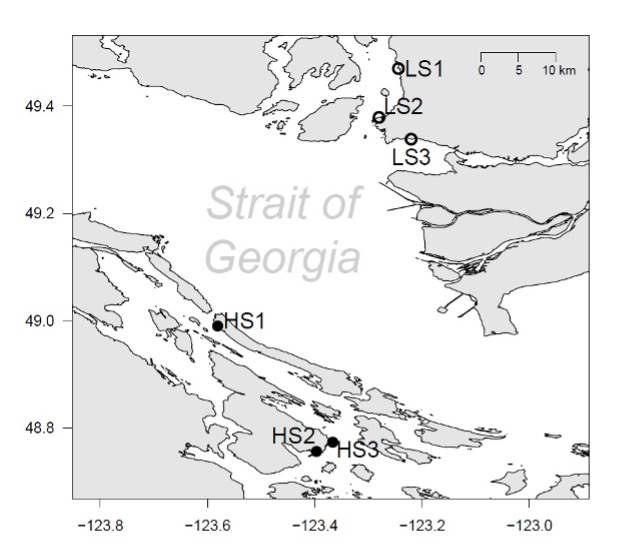
\includegraphics{/Users/sandraemry/Documents/coyle/SalinityandLimpets/figures/site_descriptions.jpg}
  \caption{figure 1}
\end{figure}

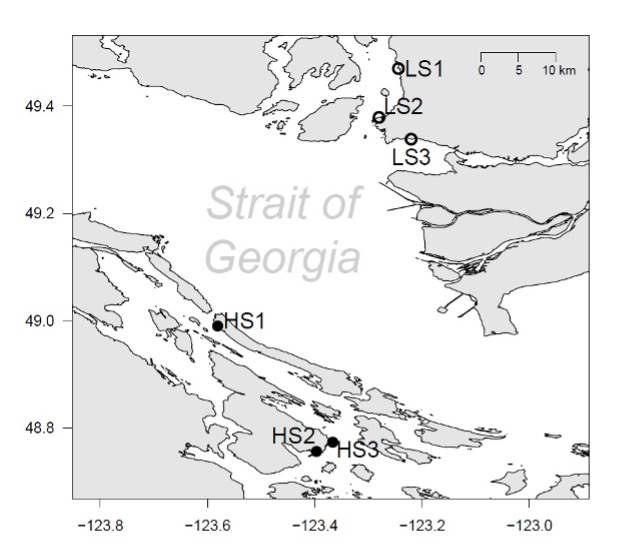
\includegraphics{/Users/sandraemry/Documents/coyle/SalinityandLimpets/figures/site_descriptions.jpg}
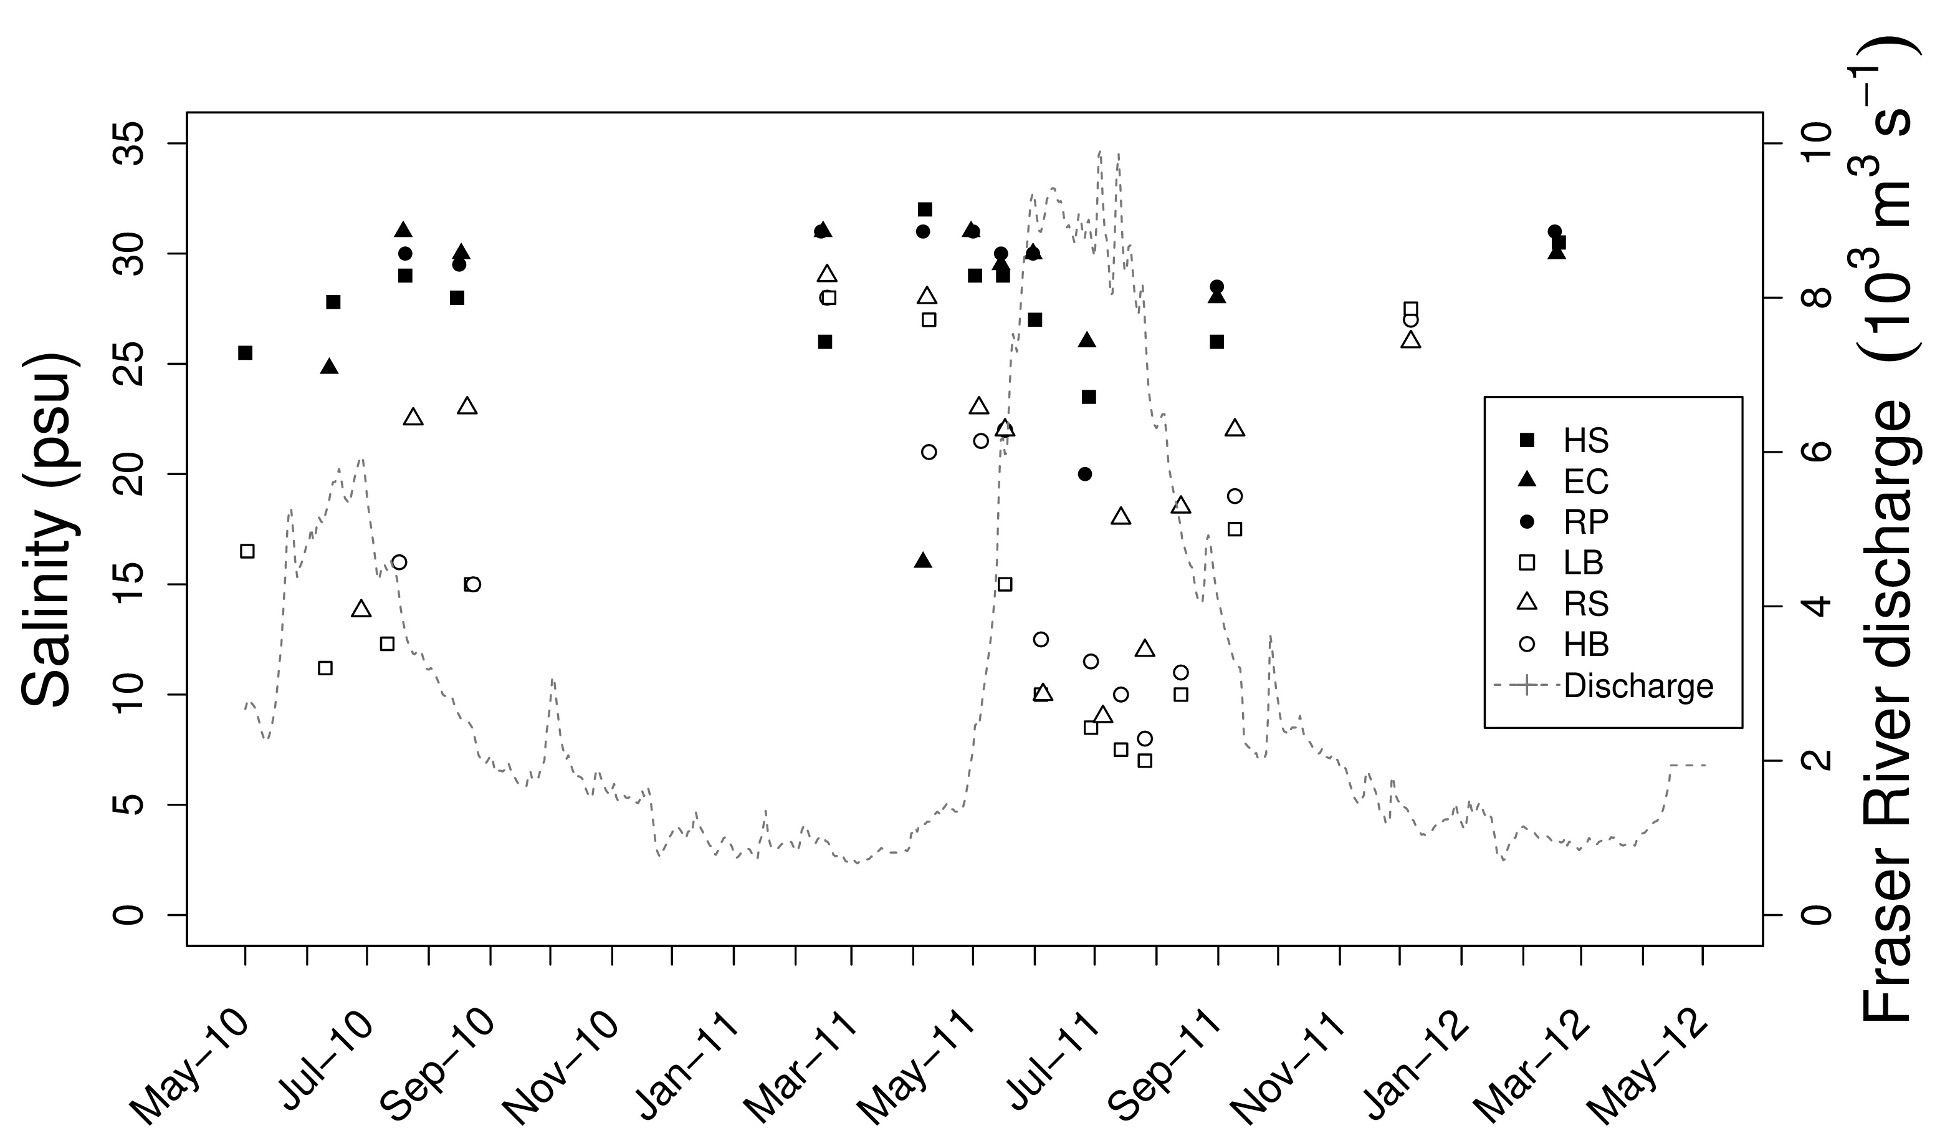
\includegraphics{/Users/sandraemry/Documents/coyle/SalinityandLimpets/figures/site_salinity.jpg}

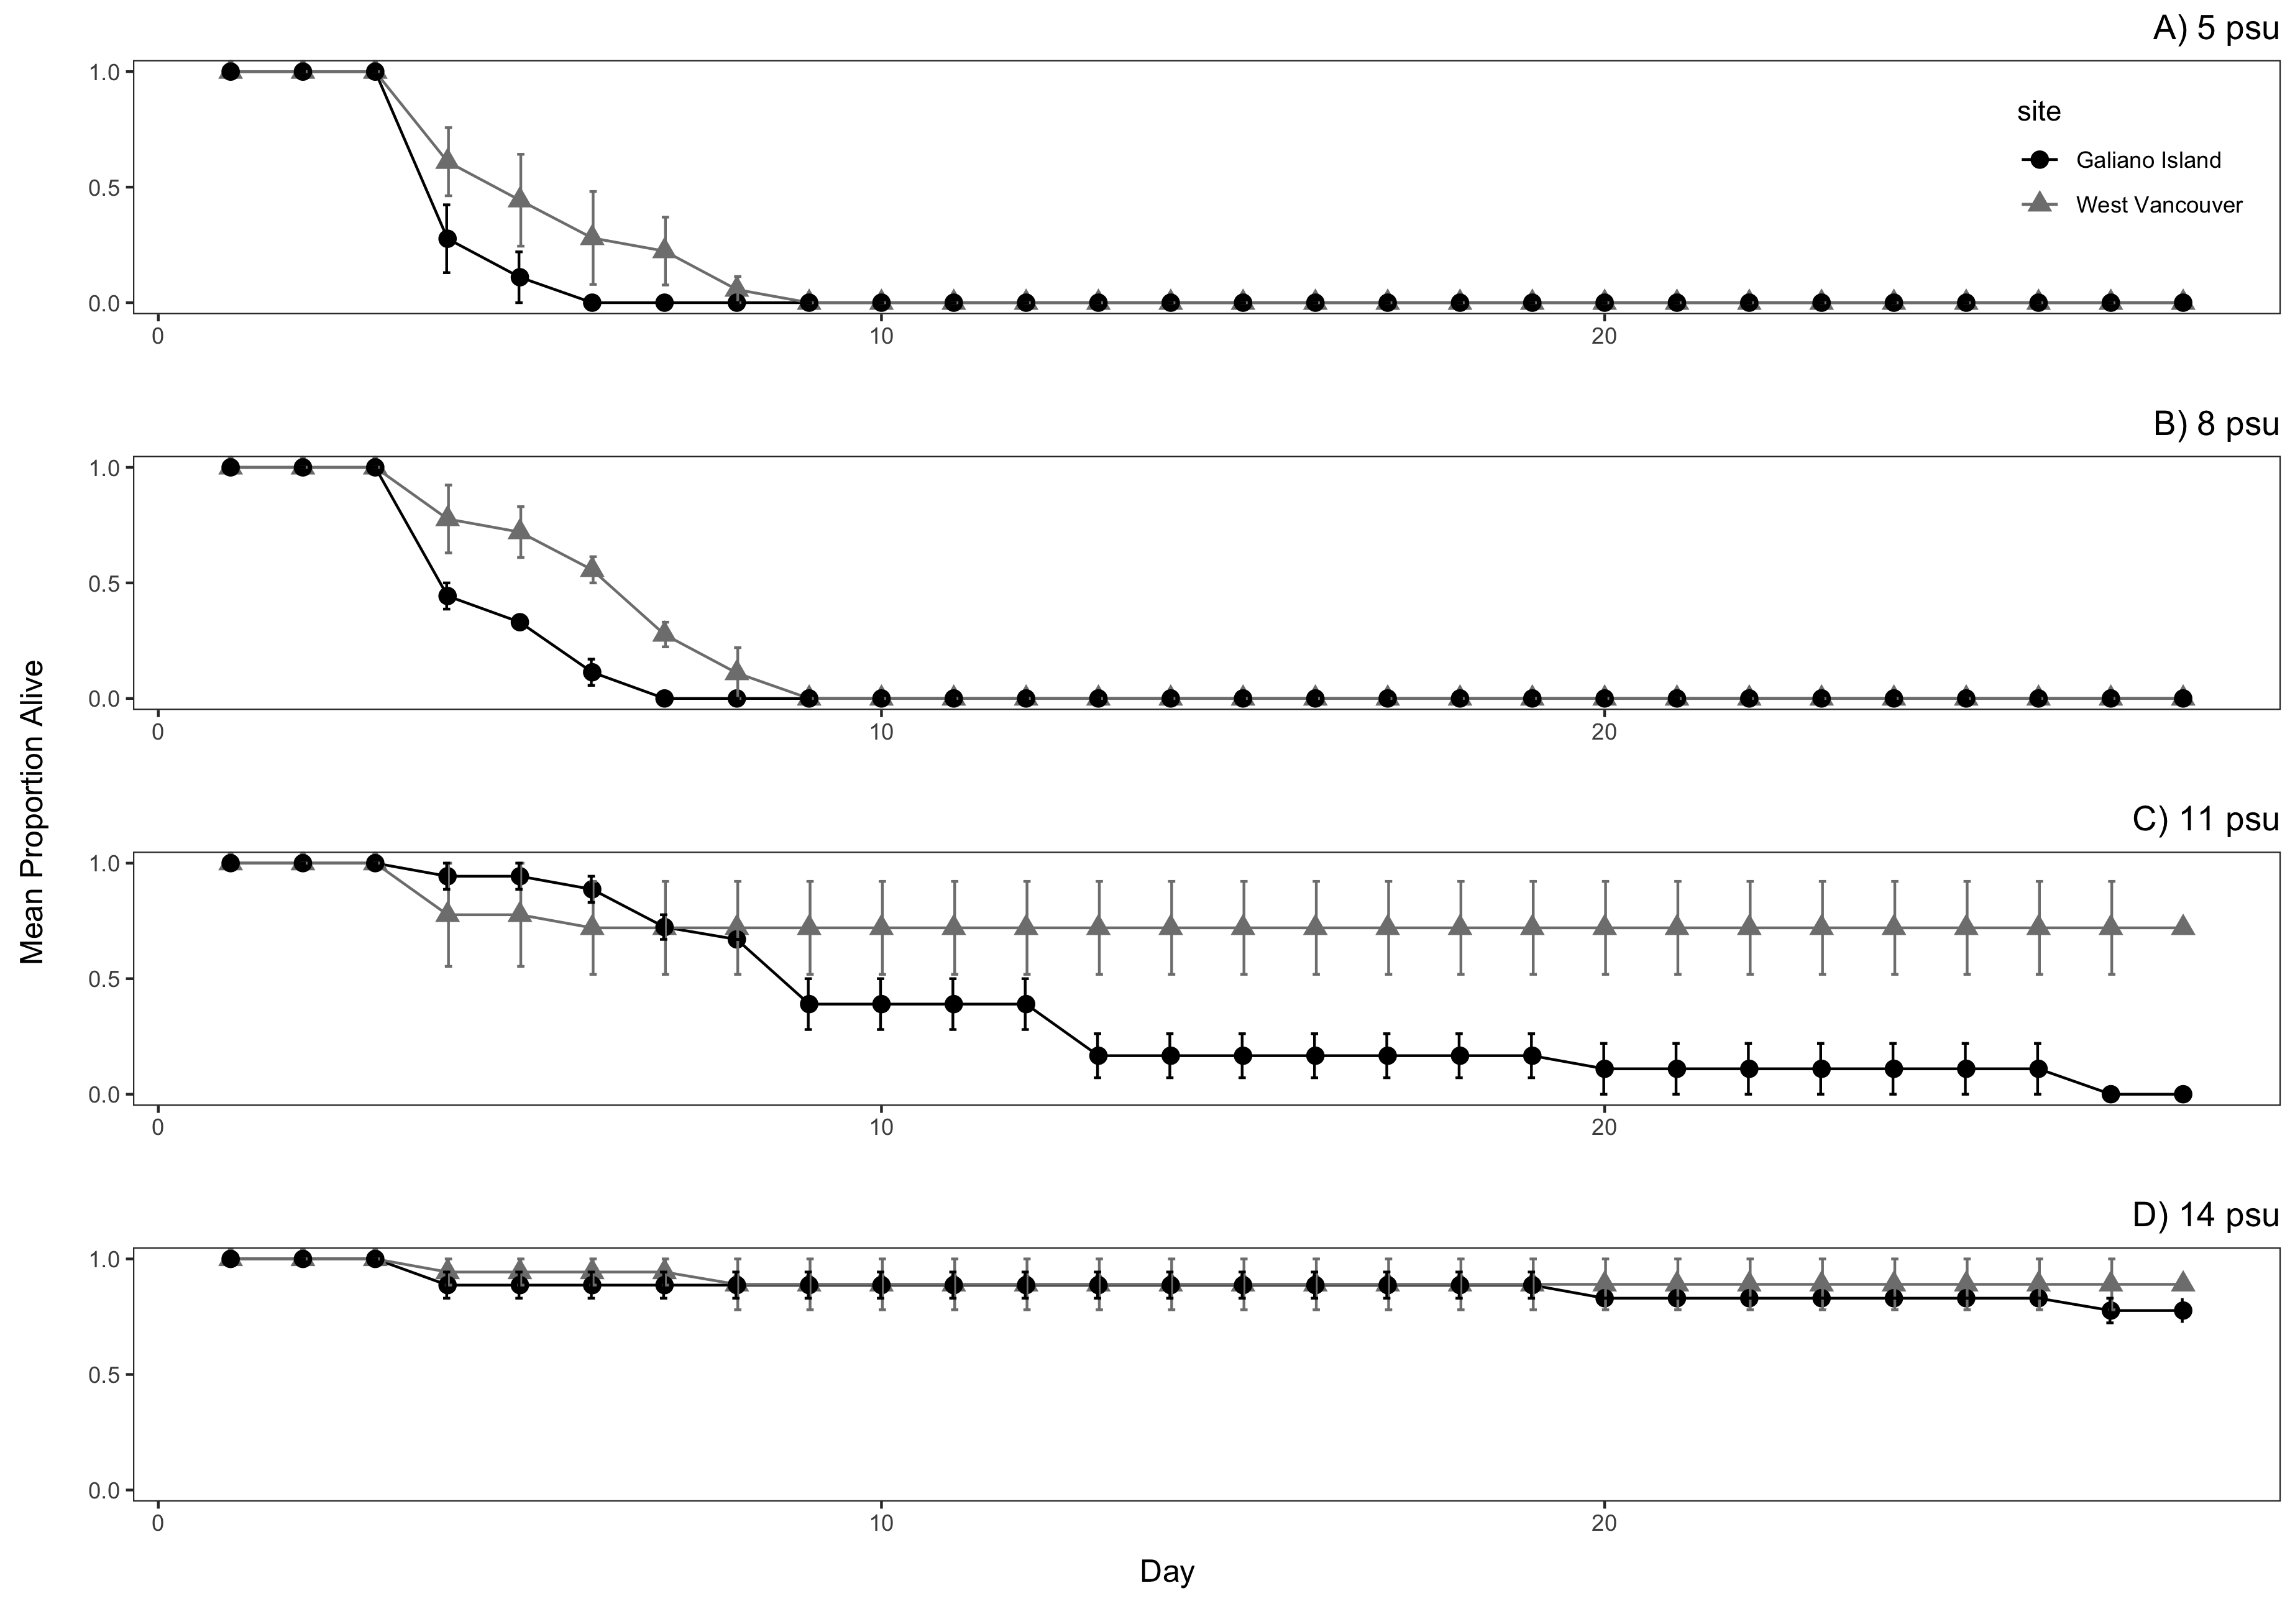
\includegraphics{/Users/sandraemry/Documents/coyle/SalinityandLimpets/figures/limpet_mortality_local_adaptation.png}
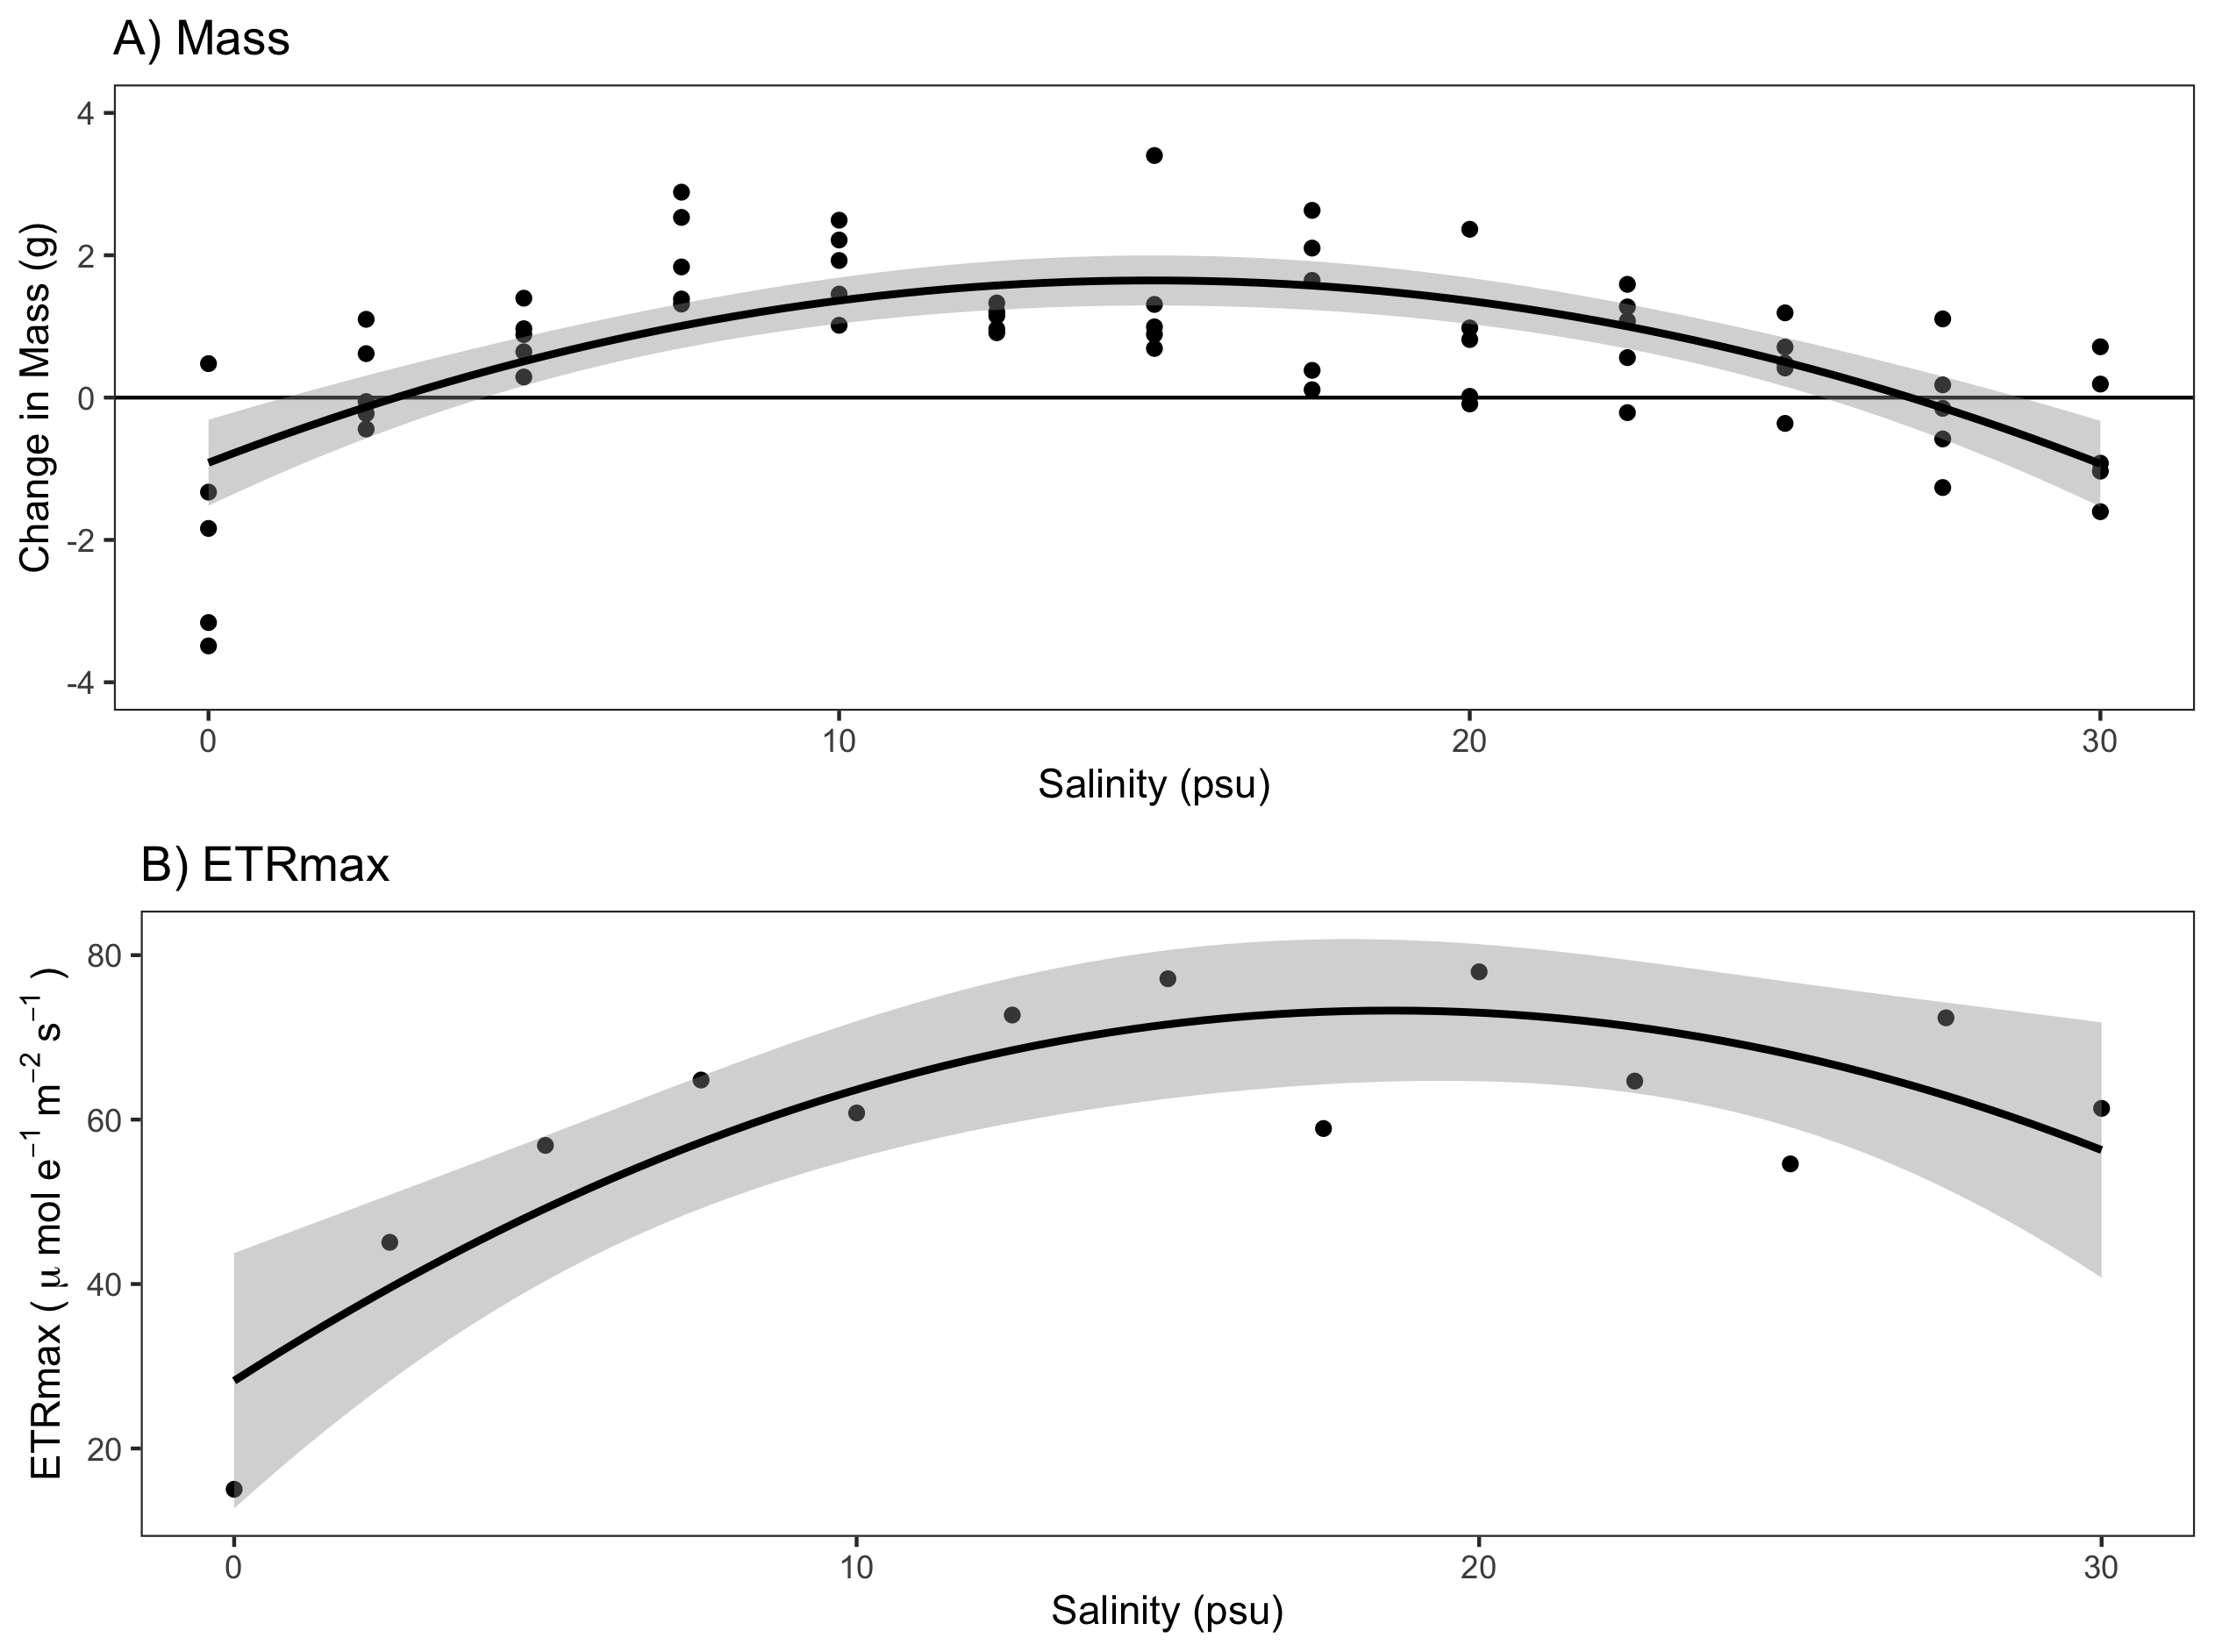
\includegraphics{/Users/sandraemry/Documents/coyle/SalinityandLimpets/figures/ulva_tolerance.png}

\end{document}
